\section{Selection methods}

\subsection{Roulette Wheel}

The roulette wheel is a selection method which attempts to apply weights to given individuals in a mating pool. The greater the weight an individual has the more likely it is to be selected, however, it also allows for individuals with less weight to be selected, though this is less likely it is still possible.

The first step in the roulette wheel selection method is assigning weights based on the fitness of an individual. We must first decide whether we want to maximize the weights or minimize the weights. For example, if out problem involves finding the minimum result then we would use the minimum technique. If we want to find the maximum result we would use the maximum technique. For this project, we are using TSP which would take advantage of the minimization technique. 

To find the minimum weights we divide 1 by the fitness using the algorithm below

\begin{equation}\label{eq:original-formula}
weight_i = 1 / fitness_i
\end{equation}

\begin{figure}[h!]
\vspace{-5pt}
\centering
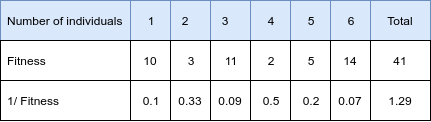
\includegraphics[width=1.0\textwidth]{images/roulette-wheel-1.png}
\caption{\label{fig:3col_graph}Minimization selection}
\end{figure}

Next, we generate a wheel which may look like below

\begin{figure}[h!]
\vspace{-5pt}
\centering
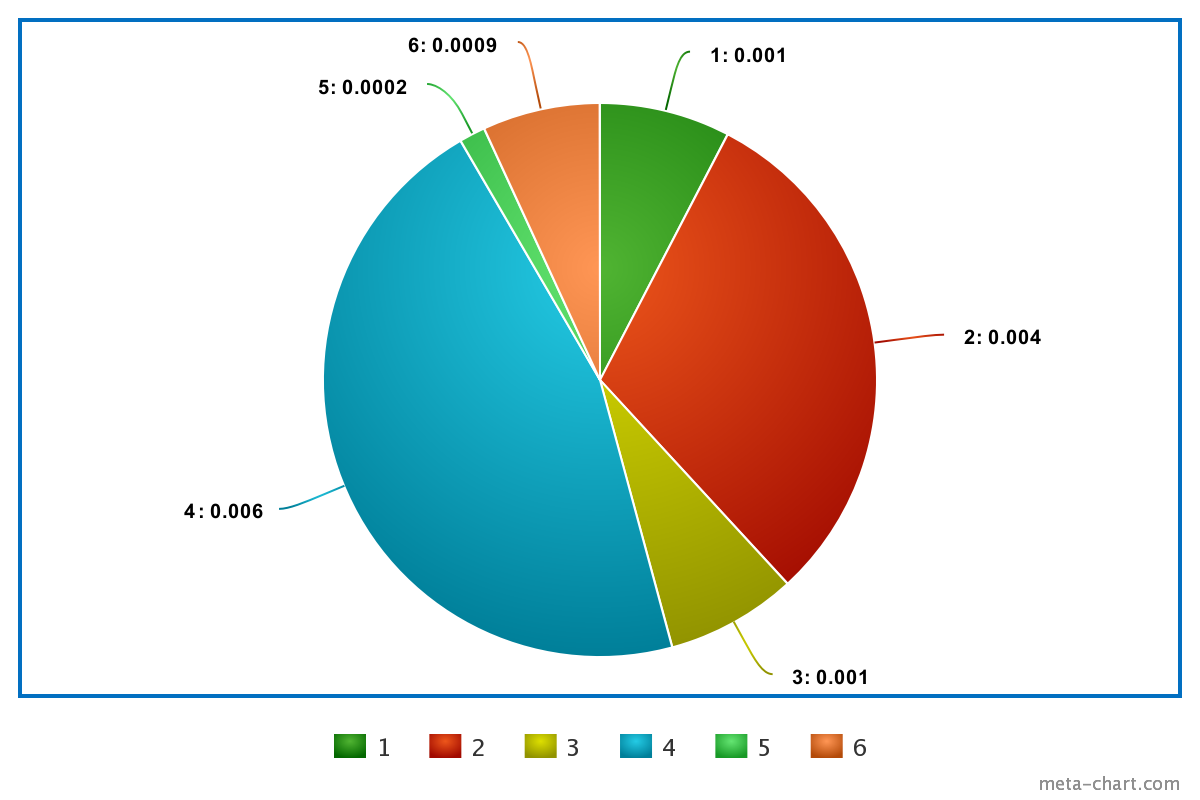
\includegraphics[width=1.0\textwidth]{images/roulette-wheel-2.png}
\caption{\label{fig:3col_graph}Roulette wheel weigths}
\end{figure}

As we can see from the image above number 4 has the most weight so is more likely to be selected. Number 5, however, has less weight, hence is very unlikely to be selected. Finally, we spin the wheel and see where it lands. This involves generating a random number and finding where it lies on the wheel.

\subsection{Best and second best}

Best and second best is relatively straightforward. The idea is to take each individual in the mating pool and order them from best to worst based on their fitness value. The top two individuals are chosen. This incurs a slight overhead in that the mating pool needs to be sorted, so it is best to use an optimized sorting technique such as the quicksort algorithm.